\documentclass[14pt, hyperref = {colorlinks}]{beamer}
\usetheme{Boadilla}
\usepackage[T2A]{fontenc}
\usepackage[utf8]{inputenc}
\usepackage[english,russian]{babel}
\usepackage[colorlinks]{hyperref}
\usepackage{amssymb,amsfonts,amsmath,mathtext}
\usepackage{cite,enumerate,float,indentfirst}



\hypersetup{
	colorlinks=true,
	linkcolor=blue,
	filecolor=magenta,      
	urlcolor=cyan,
}
\usecolortheme{seahorse}

\setbeamercolor{footline}{fg=blue}
\setbeamertemplate{footline}{
	\leavevmode%
	\hbox{%
		\begin{beamercolorbox}[wd=.333333\paperwidth,ht=2.25ex,dp=1ex,center]{}%
			А.Е. Требушинин
		\end{beamercolorbox}%
		\begin{beamercolorbox}[wd=.333333\paperwidth,ht=2.25ex,dp=1ex,center]{}%
			Новосибирск, 2019
		\end{beamercolorbox}%
		\begin{beamercolorbox}[wd=.333333\paperwidth,ht=2.25ex,dp=1ex,right]{}%
			Стр. \insertframenumber{} из \inserttotalframenumber \hspace*{2ex}
	\end{beamercolorbox}}%
	\vskip0pt%
}

\newcommand{\itemi}{\item[\checkmark]}

\title{\small{Разработка рентгенооптических трактов экспериментальных станций первой очереди проекта ЦКП «СКИФ»}}

\author{\small{%
		\emph{Докладчик:}~Требушинин Андрей\\%
		\emph{Руководитель:}~к.ф.-м.н.~Я. В. Ракшун}\\%
	\vspace{30pt}%
	Институт Ядерной Физики
	\vspace{-15pt}%
}

\date{\includegraphics[width=0.1\linewidth]{pic/logo.jpg} \hspace{20pt}
	\includegraphics[width=0.2\linewidth]{pic/SKIFlogo.png}\\
	
	\vspace{5pt}% 
	\small{Новосибирск, 2019}}

\begin{document}

\maketitle


\small
\begin{frame}
\frametitle{Цель работы}\label{t1}
\begin{center}
	Создание проекта экспериментальных стаций первой очереди проекта <<СКИФ>>
\begin{itemize}
	\item Моделирование источников излучения \\(ондуляторы, вигглеры)
  	\item Моделирование оптических элементов \\(апертуры, монохроматоры, фокусирующие зеркала)
  	\item Создание среды для обмена информаций по проектированию
	\item Координация работы между исследовательскими группами разных институтов (ИЯФ, Институт катализа и д.р.)
\end{itemize}
\end{center}
\end{frame}

\small
\begin{frame}
\frametitle{План презентации}\label{t1}
\begin{center}
		\begin{itemize}
		\item Необходимость источников СИ в России
		\item Структура проектного офиса ЦКП <<СКИФ>>
		\item Обзор источников излучения для станций
		\item Оптические схемы станций
		\item Обсуждение результатов	
		\item Благодарности 
	\end{itemize}
\end{center}
\end{frame}

\iffalse
\small
\begin{frame}
\frametitle{Окружности и прямые}\label{t1}
\begin{figure}[h]
	\center{Синхротронный источник}
	\begin{minipage}[h]{0.50\linewidth}
		\center{\includegraphics[width=0.99\linewidth]{pic/synchrotron.png}}
		%http://www.irtnanoelec.fr
	\end{minipage}

	\hfill
	\center{Лазер на свободный электронах}
	\begin{minipage}[h]{0.50\linewidth}
		\center{\includegraphics[width=0.99\linewidth]{pic/lcls.jpg}}
		%https://portal.slac.stanford.edu
	\end{minipage}
	\end{figure}
	\raggedright\tiny{\href{http://www.irtnanoelec.fr}{ссылка на рисунок сверху}}\\
	\raggedright\tiny{\href{https://portal.slac.stanford.edu/sites/conf_public/lclsiihe2018/PublishingImages/Forms/AllItems.aspx}{ссылка на рисунок снизу}}
\end{frame}
\fi

\small
\begin{frame}\label{r3}
\frametitle{Карта ускорительных центров}
\begin{figure}[h]
		\center{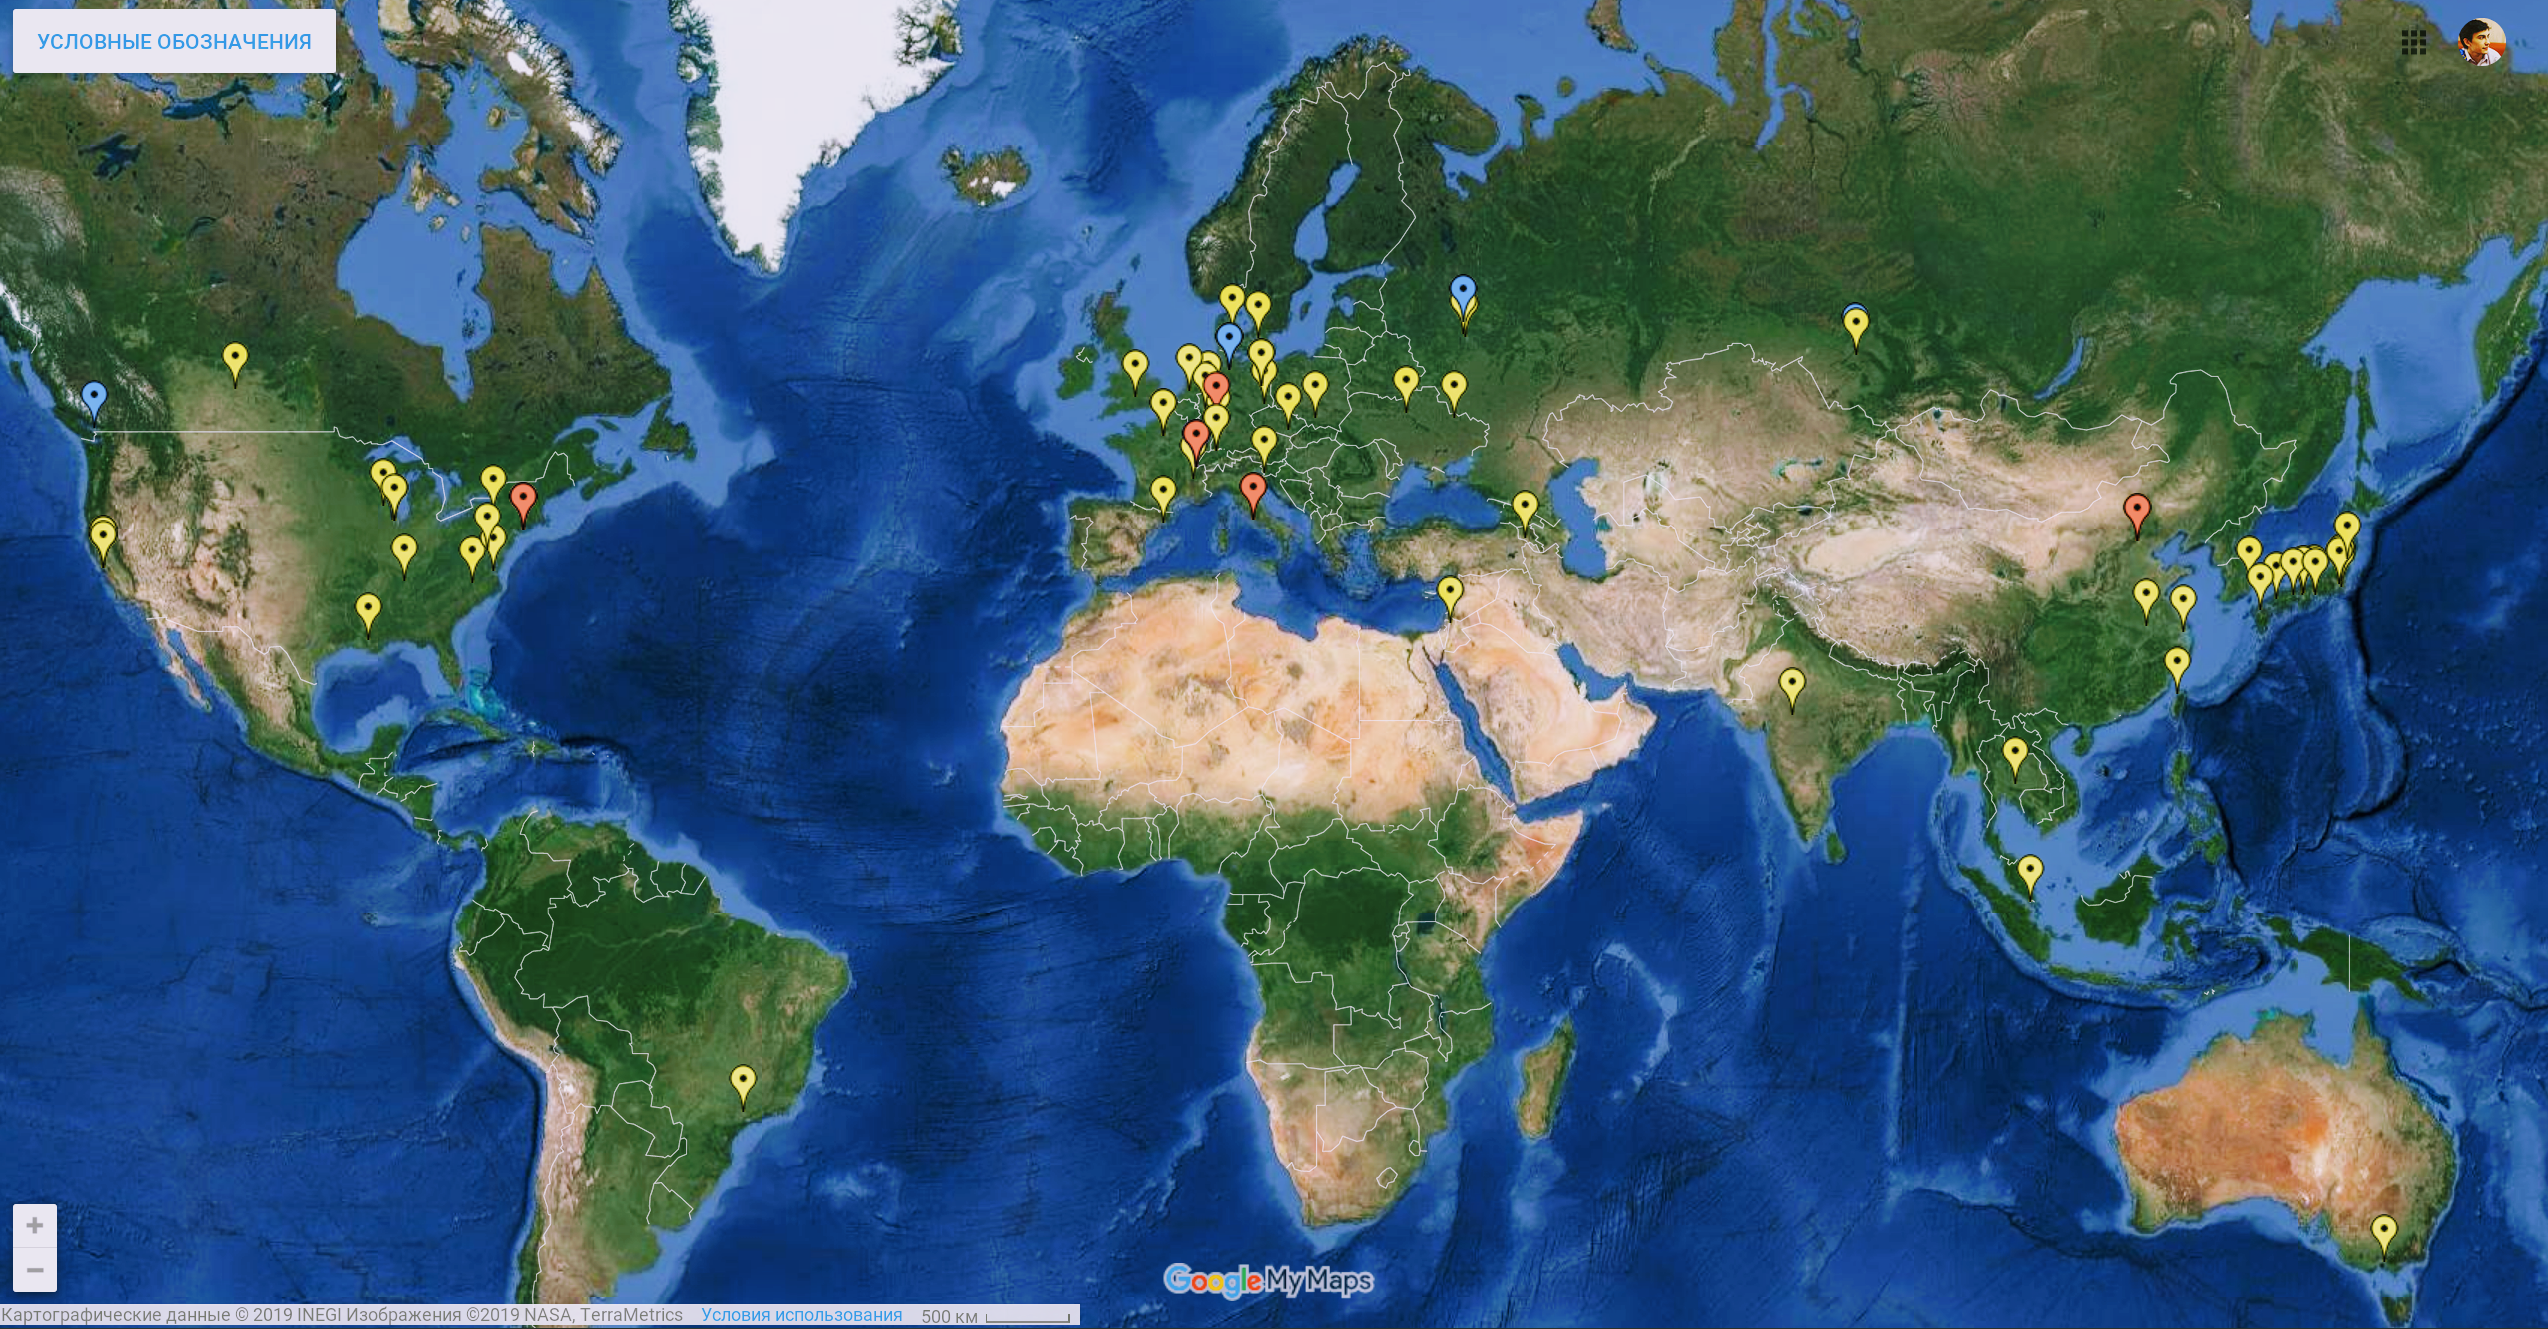
\includegraphics[width=1.0\linewidth]{pic/map.png}}	
		\raggedright\tiny{Жёлтым цветом обозначены центры синхротронного излучения}
\end{figure}
\end{frame}

\small
\begin{frame}
\frametitle{Сибирский кольцевой источник фотонов}\label{t1}
\begin{figure}[h]
	\center{}
	\begin{minipage}[h]{0.85\linewidth}
		\center{\includegraphics[width=0.99\linewidth]{pic/SKIF_2_2.png}}
		%http://www.irtnanoelec.fr
	\end{minipage}
	
	\hfill
	\center{}
	\begin{minipage}[h]{0.85\linewidth}
		\center{\includegraphics[width=0.99\linewidth]{pic/SKIF_1_2.png}}
		%https://portal.slac.stanford.edu
	\end{minipage}
\end{figure}
\end{frame}


\small
\begin{frame}
\frametitle{Структура синхротрона}\label{t1}
\begin{figure}[h]
	\center{\includegraphics[width=0.9\linewidth]{pic/outline.pdf}}	
\end{figure}
\end{frame}


\small
\begin{frame}
\frametitle{Оптическая группа ЦКП <<СКИФ>>}\label{t1}
\begin{figure}[h]
	\center{\includegraphics[width=0.8\linewidth]{pic/scheme.pdf}}	
\end{figure}
\end{frame}

\small
\begin{frame}
\frametitle{Вставные устройства. Ондуляторы.}\label{t1}
\begin{figure}[h]
\end{figure}
\end{frame}

\small
\begin{frame}
\frametitle{Ондуляторы как интерференционное устройство}\label{t1}
\begin{figure}[h]
\end{figure}
\end{frame}


\small
\begin{frame}
\frametitle{Спектр ондулятора}\label{t1}
\begin{figure}[h]
\end{figure}
\end{frame}

\small
\begin{frame}
\frametitle{Угловое распределение}\label{t1}
\begin{figure}[h]
\end{figure}
\end{frame}

\small
\begin{frame}
\frametitle{Схема ондулятора для станции 1-4}\label{t1}
\begin{figure}[h]
\end{figure}
\end{frame}

\small
\begin{frame}
\frametitle{Оптическая схема станции 1-1}\label{t1}
\begin{figure}[h]
\end{figure}
\end{frame}

\small
\begin{frame}
\frametitle{Результаты}\label{t1}
\begin{figure}[h]
\end{figure}
\end{frame}

\small
\begin{frame}
\frametitle{Благодарности}\label{t1}
\begin{figure}[h]
\end{figure}
\end{frame}

\begin{frame}
\begin{center}
	\textbf{Благодарю за внимание}
\end{center}
\end{frame}

\small
\begin{frame}
\frametitle{Скрытые файлы}\label{t1}
\begin{figure}[h]
\end{figure}
\end{frame}



\end{document}
